\documentclass{article}

\usepackage[margin=1in]{geometry} 
\usepackage[english]{babel}
\usepackage[T1]{fontenc}
\usepackage[utf8]{inputenc}
\usepackage{amsmath,amsthm,amssymb,amsfonts, fancyhdr, color, comment, graphicx, environ}
\usepackage{xcolor}
\usepackage{mdframed}
\usepackage[shortlabels]{enumitem}
\usepackage{indentfirst}
\usepackage{hyperref}
\usepackage{lastpage}
\usepackage{listingsutf8}
%\usepackage{ff++listings}
\usepackage{amsmath}
\DeclareMathOperator{\Tr}{Tr}

\usepackage{physics}
\usepackage{amsfonts}
\usepackage{float}
\PassOptionsToPackage{hyphens}{url}\usepackage{hyperref}

\newenvironment*{remerciements}{%
\renewcommand*{\abstractname}{Acknowledgements}
\begin{abstract}
}{\end{abstract}}

\usepackage{xurl}

\renewcommand{\footrulewidth}{0.8pt}
\hypersetup{
    colorlinks=true,
    linkcolor=blue,
    filecolor=magenta,      
    urlcolor=blue,
}

\pagestyle{fancy}

\newenvironment{problem}[2][Etape]
    { \begin{mdframed}[backgroundcolor=gray!20] \textbf{#1 #2} \\}
    {  \end{mdframed}}

\newenvironment{solution}{\textbf{Réponse}}

\lhead{Florent Pollet}
\rhead{ES2A EEP-02} 
\chead{\textbf{Vaccine strategies}}
\lfoot{Véronique Stoven}
\cfoot{Mines Paris}
\rfoot{\thepage/\pageref*{LastPage}}


\let\up\textsuperscript

\usepackage{biblatex}
\addbibresource{biblio/biblio.bib}

%\usepackage[backend=bibtex]{biblatex}
\usepackage[nottoc, notlof, notlot]{tocbibind}

\begin{document}

    \title{\Large ES2A EEP-02  \\[0.5cm]
        \bf\Large Vaccine strategies}
\author{\large Florent Pollet \ \\}
\date{\large\today}

\makeatletter
    \begin{titlepage}
        \begin{center}
	   { 
\includegraphics[width=12cm]{imgs/mp_logo.png}}
	   {\ \\ \ \\}
        \vbox{}\vspace{2cm}
            {\@title }\\[1cm] 
            %{ \includegraphics[width=7cm]{imgs/cover.PNG}}\\[1cm]
            {\@author}

            {\large \ \\ Supervisor: \bf Véronique Stoven\\ \ \\}
            {\@date\\}

        \end{center}

        \vspace{4cm}
        \begin{figure}[H]
            \centering
            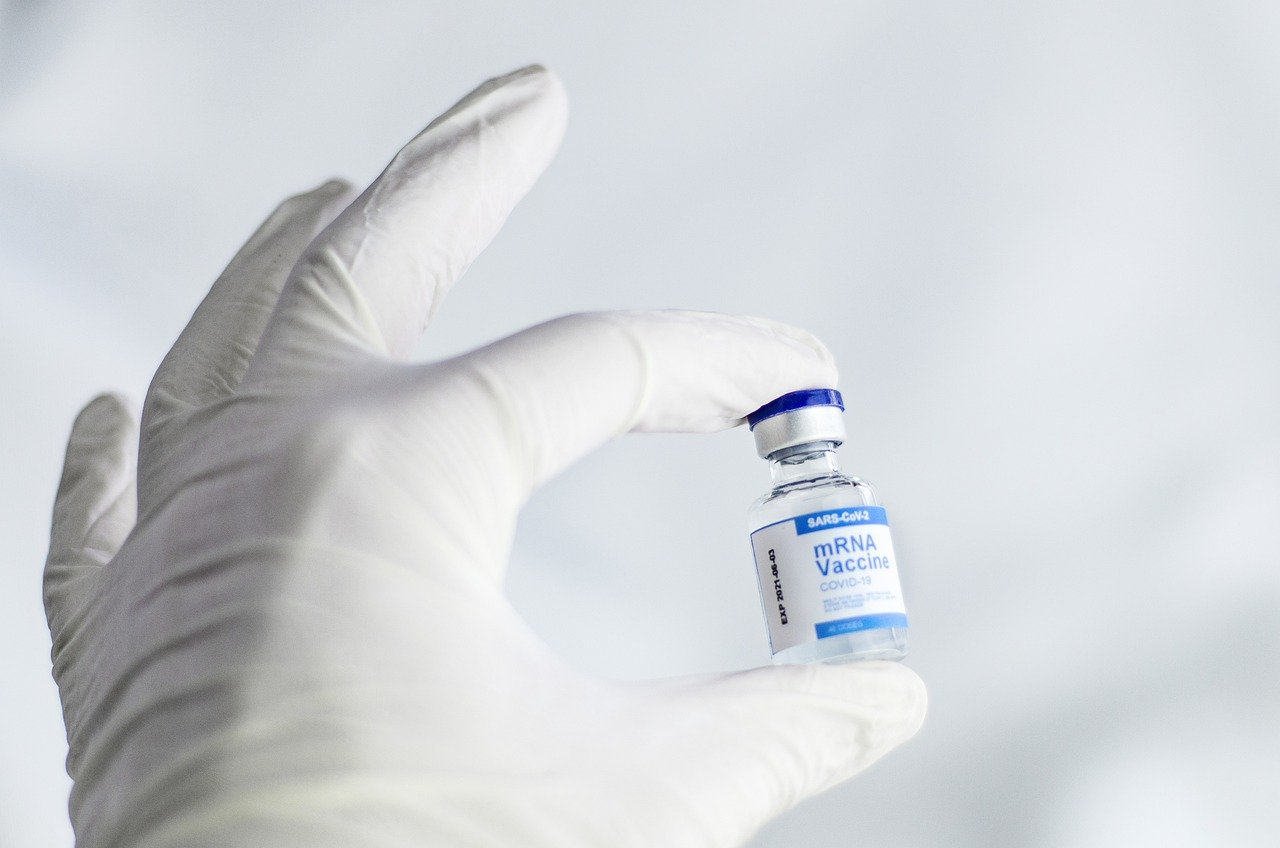
\includegraphics[width=0.4\textwidth]{imgs/vaccineCover.jpg}
        \end{figure}

    \end{titlepage}


    \begin{abstract}        
        In a context of a pandemic and major doubts towards vaccination among populations, this paper deals with vaccine strategies, especially how mRNA vaccines are revolutionizing them.
        It is clear that immunology represents a complex field of science,
            and nowadays the breakthroughs in biotechnologies are offering new possibilities to accelerate vaccine development, efficiency and safety as well as a better understanding
            our immune system.
        This paper aims at summarizing the different vaccine techniques with a special attention to mRNA vaccines\footnote{Messenger RiboNucleic Acid}, in order to
            have an overview of the current vaccine strategies which are going to evolve.
        % implications, finding, methods ? go further ?
    \end{abstract}

        
    \begin{remerciements}
        I cannot express enough thanks to my teacher Véronique Stoven for her interesting lessons about molecular and synthetic biology,
            which inspired me this topic.
        I absolutely loved doing research and writing this report.
    \end{remerciements}


    \tableofcontents


    \newpage

    \makeatother

    \section{Introduction}

    Vaccines represent an amazing invention which saved millions of lives in the world since 2000 \autocite{HowManyLives2021}.
    Even if vaccination is not new, the recent pandemic of COVID-19 brought to the forefront this field, generating great advances but also important debates about safety, ethics and politics.
    It is necessary to take into account all these changes and to adapt to be avoid a backward step and the rejection of these opportunities. 
    
    Therefore it would be interesting to better understand the recent evolutions in vaccine strategies and technologies and the consequences it may have on society.
    
    Firstly, I will briefly recall the history of vaccination, detailing the different types of vaccines which have been developed.
    Secondly, I will present the technology of mRNA (messenger ribonucleic acid) vaccines which are currently the main source of progress.
    Thirdly, I will observe how society is integrating these developments and what issues remain to be solved.

    This theme is closely linked to the mechanics of the immune system, in medicine, which will not be detailed in this article due to the needed knowledge in medicine.
    In any case, I would like to thank Ms. Stoven for her molecular biology course and her help in the writing of this article.

    %Blabla. Belle oeuvre : \autocite{zhangMulticladeEnvGag2021}, blabla.

    \section{A brief history of vaccines}

        \subsection{Discovery of the principle}

            The principle of vaccination could come from the idea of mithridatism, that is to say the ability to gain protection against a poison by taking several benign amounts.
            
            Variolization, which corresponds to injecting smallpox pustules to gain immunity against smallpox, began in China around the 10\up{th} century \autocite{canouiHistoryPrinciplesVaccination2019}. 
            Before the scientist Jenner, several persons realized variolization in England. However, in 1798, this is Jenner who made a link between cowpox and smallpox: 
                cowpox could an attenuated version of smallpox.            

            The idea of vaccination is to create an individual, long-term and efficient protection against a pathogen (like a virus or a bacteria), without causing serious symptoms.
            This is made possible thanks to the memory of human's immune system.

            \subsubsection{A quick look on the immune system}



            % variole eradication

            % lymphocyte T & B mémoire

        \subsection{First generation of vaccines}
            
            It is only between 1870 and 1885 with Pasteur's works, that the first vaccines were developed.

        \subsection{Second generation of vaccines}

        \subsection{Towards a third generation}

        % not only prophylathic but therapeutic

    \section{mRNA vaccines: a promising technology}

        \subsection{Principle}

        \subsection{Development}

        \subsection{Advantages and drawbacks}

    \section{New stakes for vaccines in the 21\up{st} century}

        \subsection{World inequalities}

        \subsection{Public policies}

        \subsection{New uses and technical challenges}

    \section{Conclusion}

    % science is not enough
    % rabelais
    % vaccine acceptance is as important as vaccine development

    % what is a vaccine ?

    % a short history : first generation (whole-organism vaccines), second generation (reduce risks from live vaccines = subunit vaccines/toxoid/recombinant),
                        % third generation (RNA/DNA vaccine)
                        %In 2021, Katalin Karikó and Drew Weissman received Columbia University's Horwitz Prize for their pioneering research in mRNA vaccine technology
                        %operatioin warm speed

    % monovalent & polyvalent (more complex : interferences, strength of the immune response)
    % only student monovalent
    % only nanogram or microgram immogen
    % adjuvant (alum) to boost or to store (preservatives, thiomersal/phenoxyethanol, formaldehyde in influenza) -> risk of allergy
    %% excipients also : antibiotics, egg protein, kill 
    % names : abbreviation

    % legislation
    % patent : stakes : licensing
    % vaccine acceptance by population (save live, economic)
    % manufacturing, distribution, losgitical factor : prioritize
    % state role and WHO role
    % record for adverse eeffects...
    % EMA/FDA



    % which phase for a vaccine development
    %scientific and then safety 
    % use and scheduling ? many vaccine when young, need combination of injections
    % different  phases
    % paradox of economic development of vaccines : role of government, universities and non-profit organizations
    % need infrastructure and workforce
    % The large number of vaccines and boosters recommended (up to 24 injections by age two) has led to problems with achieving full compliance.
    % to healthy people : huge quality needed
    % build : bioreactor
    % vials = flacons
    % filling vials : difficult step

    % key players & firms
    % 10/15 years official development
    % from injection to oral vaccines (ouverture)

    % link to veterinary medicine

    % revoir test ELISA principe
    % next stakes : vaccine resistance (same as antimicrobial resistance) (immune evasion) -> covid, this is the case, if total protection less likely than only against serious forms
    % transgenic plant
    

    %https://biontech.de/covid-19-portal/mrna-vaccines (interesting schema)
    %https://sitn.hms.harvard.edu/flash/2015/rna-vaccines-a-novel-technology-to-prevent-and-treat-disease/
    % Bill & Melinda Gates Foundation invested $53 million in the German company, CureVac, which specializes in the development of these vaccines
    % perspective for the future as regard influenza vaccines : influenza vaccine, whereas the company CureVac claims that RNA-based vaccines could be manufactured in less than two months at a lower production cost, (harvard) + cancer vaccines
    %

    \newpage

    \appendix

    \section {Source code}
    The source code of this document is available at \url{https://github.com/florian6973/biology-report}.
    
    \nocite{*}
    \printbibliography
    
\end{document}